\section{The cavity lower bound}\label{sec:cavity}

The cavity comparison belongs to the variational approach of
Aizenman, Sims, and Starr \cite{ASS2003}. Here the reservoir and added
coordinates are coupled through fresh directions in the spectral
eigenspaces; the rotation and quadratic-tilt identities required by this
coupling are derived below.

We now prove the lower bound for a finite spectral alphabet with positive
rational proportions.  We compare systems of sizes $N$ and $N+n$, where
$n$ is fixed and $s_a:=n\rho_a$ is integral for every $a$.  The comparison
must retain the base interaction: its eigenspaces contain the fresh
directions that become Gaussian cavity variables.  After evaluating the
resulting change of measure, site symmetry will identify its field as a
maximizer in the definition of $S$.

Fix a progression of dimensions with step $n$ and group counts satisfying
\begin{equation}\label{cav:counts}
 k_a(N+n)=k_a(N)+s_a,
 \qquad \frac{k_a(N)}{N}\longrightarrow\rho_a.
\end{equation}
All limits and uniform bounds in this section concern sufficiently large
dimensions on this progression, with the alphabet, its proportions, and
$n$ fixed.  We use the unenriched perturbations of Section~\ref{sec:rotation}
at $t=1$.  Write $\theta=(u,v)$ for their parameters, $\eta$ for the
product uniform probability on their parameter space, and
\[
 Z_N^\theta=\text{the perturbed partition function},\qquad
 \mathcal F_N(\theta)=\E\log Z_N^\theta.
\]
The cube prior in $Z_N^\theta$ remains its uniform probability.
Proposition~\ref{rot:gg} supplies measurable sets $\mathcal G_N$ with
$\eta(\mathcal G_N)\to1$ such that every sequence
$\theta_N\in\mathcal G_N$ has, after extraction, joint GG limits with
fixed spectral diagonals.  We first bound the increments at any such
sequence, and average over parameters only at the end.

\subsection{A coupling that preserves the base law}

Let $E:\R^n\to\R^{N+n}$ embed the last $n$ coordinates, and let
$P_a^+$ be the full spectral projectors.  Define
\[
 M_a=E^{\mathsf T}P_a^+E,\qquad
 d=(m-1)n.
\]
The matrices $M_a$ converge in probability to $\rho_a I_n$, and are
positive definite almost surely for all sufficiently large dimensions.
The first assertion follows from rotational symmetry and concentration;
the second follows, for example, by representing a uniform frame with
independent Gaussians.  Throughout, zero-dimensional complementary
spaces have the usual empty-matrix conventions.

\begin{lemma}[Coupled interaction and fresh frames]\label{cav:coupling}
There is a coupling of the full interaction of size $N+n$ and an
interaction of size $N$ with the spectral counts in \eqref{cav:counts}
with the following properties.  There are $d$ orthonormal special axes
in the first $N$ coordinates and matrices
\begin{equation}\label{cav:blocks}
 \begin{pmatrix}A_N&L_N\\L_N^{\mathsf T}&C_N\end{pmatrix}
 \longrightarrow
 \begin{pmatrix}A&L\\L^{\mathsf T}&C\end{pmatrix}
 \quad\text{in probability},
 \qquad C=\Big(\sum_a\rho_a\lambda_a\Big)I_n,
\end{equation}
where $A_N,A$ act on $\R^d$.  Fix a diagonal matrix $A_0$ with
$n-s_a$ copies of $\lambda_a$.  If $y\in\R^d$ is the projection of a
base spin $\sigma$ onto the special axes, then adjoining
$\varepsilon\in\{-1,1\}^n$ changes the main exponent by
\begin{equation}\label{cav:factor}
 \log W_N(y,\varepsilon)
 =\frac12y^{\mathsf T}(A_N-A_0)y
   +y^{\mathsf T}L_N\varepsilon
   +\frac12\varepsilon^{\mathsf T}C_N\varepsilon.
\end{equation}
Conditional on the base spectral projectors, the special axes assigned
to group $a$ form a uniform orthonormal $(n-s_a)$-frame in that group.
They may be taken independent of the base perturbations given those
projectors.  For finitely many base replicas, their projection variables
converge jointly with any overlap limit to centered Gaussian marks,
independent across the axes conditional on the overlap array, with
covariance $A^a_{lj}/\rho_a$ for an axis assigned to group $a$.
Moreover, for every fixed $q>0$,
\begin{equation}\label{cav:base-moments}
 \sup_{N,\theta}\E\langle |y|^q\rangle_{N,\theta}<\infty.
\end{equation}
Here the brackets denote the base Gibbs probability and the expectation
also includes the special frames.
\end{lemma}

\begin{proof}
The mutually orthogonal spaces $\operatorname{ran}(P_a^+E)$ have
orthonormal coordinate maps $P_a^+E M_a^{-1/2}$.  In their direct sum,
the cavity coordinate map is the vertical stack $(M_a^{1/2})_a$.
Its columns are orthonormal because $\sum_aM_a=I_n$.  Complete these
columns to an orthonormal basis, with the complement first, using a rule
continuous near the limiting stack $(\sqrt{\rho_a}I_n)_a$.  One may
project a fixed limiting complementary frame and orthonormalize it.
In these coordinates the interaction is the left matrix of
\eqref{cav:blocks}.  Its limit is a conjugate of
$\bigoplus_a\lambda_a I_n$, with cavity column blocks
$\sqrt{\rho_a}I_n$.  This proves \eqref{cav:blocks}.

The complement to the cavity coordinates in this direct sum lies in
the first $N$ coordinates and has dimension $d$; its chosen basis gives
the special axes.  All other eigenvectors also lie in the first $N$
coordinates, with multiplicities $k_a(N+n)-n$.  Retain them and assign
$A_0$ to the special axes.  The resulting base multiplicity is
\[
 k_a(N+n)-n+(n-s_a)=k_a(N+n)-s_a=k_a(N).
\]
The geometric decomposition is thus
\begin{equation}\label{cav:decomposition}
 \R^{N+n}
 =\MathActualText{2A01005F00610020211B005F00610020002800640069006D0020003D0020004E00202212002000640029}{\underbrace{\bigoplus_a\mathcal R_a}_{\dim=N-d}}
   \mathbin{\oplus}
   \MathActualText{D835DCB1005F004E0020002800640069006D0020003D002000640029}{\underbrace{\mathcal V_N}_{\dim=d}}
   \mathbin{\oplus}
   \MathActualText{0045211D005E006E0020002800640069006D0020003D0020006E0029}{\underbrace{E\R^n}_{\dim=n}},
 \qquad
 \mathcal R_a=\operatorname{ran}P_a^+\cap\ker E^{\mathsf T}.
\end{equation}
The base interaction agrees with the full interaction on the first
summand and uses $A_0$ on $\mathcal V_N$.  Subtracting the two quadratic
forms gives \eqref{cav:factor}.

Conditional on $(M_a)_a$, rotations of the first $N$ coordinates act
transitively on the remaining frame and subspace data.  Their conditional
law is therefore the invariant probability on this orbit.  In
particular the base interaction has its Haar law, independently of
$(M_a)_a$.  After conditioning further on the base projectors, the
remaining freedom is the product of the rotations within their
eigenspaces.  The selected axes consequently have the asserted uniform
frame law.  Generate the base perturbations independently conditional
on the projectors, using their prescribed Gaussian kernels.  This
preserves that conditional frame law; no full-system Gaussian
coefficient realization is inherited by the base.

For a uniform unit vector in a group of dimension $k_a(N)$, its
projections on fixed replicas have covariance
\[
 \frac{(\sigma^l)^{\mathsf T}P_a\sigma^j}{k_a(N)}
 =\frac{N}{k_a(N)}A^a_{lj}.
\]
Generate the fixed number of selected vectors by independent Gaussian
vectors divided by $\sqrt{k_a(N)}$, then orthonormalize them.  Their
Gram matrix tends to the identity.  Before orthonormalization the
replica projections are already jointly Gaussian with the displayed
covariances, which are uniformly bounded.  The Gram correction thus
does not change the limit.  The sphere moment formula, or Gaussian
radial independence, gives every fixed moment uniformly, since
$\|P_a\sigma\|\le\sqrt N$ and $k_a(N)/N$ stays bounded below.  This
proves \eqref{cav:base-moments} for any base Gibbs probability that is
independent of the selected frames conditional on the projectors.
\end{proof}

Figure~\ref{fig:cavity-decomposition} summarizes the shared spectral
spaces and the two interactions on the special coordinates.

\begin{figure}[tbp]
\centering
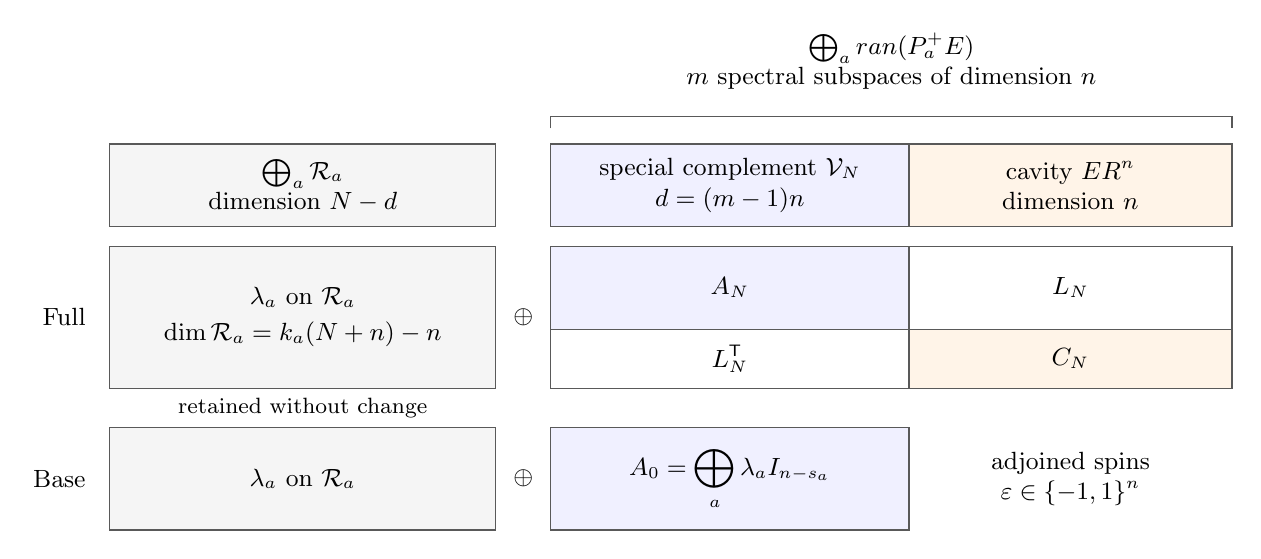
\begin{tikzpicture}[
  x=1cm,y=1cm,
  every node/.style={font=\small,align=center,inner sep=2pt},
  box/.style={draw=black!65,line width=.45pt},
  retained/.style={box,fill=black!4},
  special/.style={box,fill=blue!6},
  cavity/.style={box,fill=orange!9}
]
  \draw[black!65,line width=.45pt]
    (6.85,5.30)--(6.85,5.45)--(15.50,5.45)--(15.50,5.30);
  \node[text width=8.3cm] at (11.175,6.15)
    {$\textstyle\bigoplus_a\operatorname{ran}(P_a^+E)$\\
     $m$ spectral subspaces of dimension $n$};

  \draw[retained] (1.25,4.05) rectangle (6.15,5.10);
  \node at (3.70,4.575)
    {$\textstyle\bigoplus_a\mathcal R_a$\\dimension $N-d$};
  \draw[special] (6.85,4.05) rectangle (11.40,5.10);
  \node at (9.125,4.575)
    {special complement $\mathcal V_N$\\$d=(m-1)n$};
  \draw[cavity] (11.40,4.05) rectangle (15.50,5.10);
  \node at (13.45,4.575)
    {cavity $E\mathbb R^n$\\dimension $n$};

  \node[anchor=east] at (1.02,2.90) {Full};
  \draw[retained] (1.25,2.00) rectangle (6.15,3.80);
  \node at (3.70,2.90)
    {$\lambda_a$ on $\mathcal R_a$\\[2pt]
     $\dim\mathcal R_a=k_a(N+n)-n$};
  \node at (6.50,2.90) {$\oplus$};
  \draw[special] (6.85,2.75) rectangle (11.40,3.80);
  \draw[box] (11.40,2.75) rectangle (15.50,3.80);
  \draw[box] (6.85,2.00) rectangle (11.40,2.75);
  \draw[cavity] (11.40,2.00) rectangle (15.50,2.75);
  \node at (9.125,3.275) {$A_N$};
  \node at (13.45,3.275) {$L_N$};
  \node at (9.125,2.375) {$L_N^{\mathsf T}$};
  \node at (13.45,2.375) {$C_N$};

  \node[font=\footnotesize,inner sep=.5pt] at (3.70,1.75) {retained without change};
  \node[anchor=east] at (1.02,.85) {Base};
  \draw[retained] (1.25,.20) rectangle (6.15,1.50);
  \node at (3.70,.85) {$\lambda_a$ on $\mathcal R_a$};
  \node at (6.50,.85) {$\oplus$};
  \draw[special] (6.85,.20) rectangle (11.40,1.50);
  \node at (9.125,.85)
    {$\displaystyle A_0=\bigoplus_a\lambda_a I_{n-s_a}$};
  \node at (13.45,.85)
    {adjoined spins\\$\varepsilon\in\{-1,1\}^n$};
\end{tikzpicture}
\caption{The coupled cavity decomposition, with schematic block widths.
The full and base interactions agree on the remaining spectral spaces
$\mathcal R_a$. The span of the $m$ spectral images of the cavity
coordinates splits into the special complement and the cavity itself;
the full interaction on this span has each eigenvalue $\lambda_a$
with multiplicity $n$. Assigning $A_0$ to the special complement gives
the prescribed base multiplicities. When $m=1$, the special complement
is absent. Conditional on the base spectral projectors, the $n-s_a$
special axes assigned to group $a$ form a
uniform orthonormal frame. The base perturbations are generated
independently of these frames conditional on those projectors.}
\label{fig:cavity-decomposition}
\end{figure}


\subsection{Perturbations and bounded Gibbs tests}

The logarithmic comparison will give a lower bound involving one field
in the supremum defining $S$.  The cavity-spin tests will show that this
field is maximizing.

In averages containing $\varepsilon$, use its independent uniform
probability on the cavity cube.  Write $\langle\cdot\rangle_0$ for
this probability times the perturbed base Gibbs probability.  All
expectations below include the coupled spectral data and the special
frames.  Let $W$ denote \eqref{cav:factor} with the limiting matrices.

\begin{lemma}[Finite-size comparison]\label{cav:comparison}
There are deterministic $\delta_N\downarrow0$, uniform over the
perturbation parameters, such that
\begin{equation}\label{cav:increment-comparison}
 \mathcal F_{N+n}(\theta)-\mathcal F_N(\theta)
 \ge
 \E\log\big\langle
 W_N(y,\varepsilon)e^{-\delta_N(1+|y|^2)}
 \big\rangle_0.
\end{equation}
The right-hand side is bounded below uniformly in $N$ and $\theta$.
In addition, any bounded continuous test of the two-replica total
overlap and the cavity spins in the full system can be evaluated,
up to an error that vanishes first as $N\to\infty$ and then as
$B\to\infty$, using the base probability reweighted by
$W_N\ind_{\{|y|\le B\}}$ and the base total overlap.
\end{lemma}

\begin{proof}
We condition first on all coupled spectral data.  Outside the
special/cavity coordinates the full and base projectors coincide.
Their overlap difference, including the change of dimension divisor,
is bounded on two configurations by
\begin{equation}\label{cav:overlap-error}
 \frac{C_n}{N}\big(1+|y^1|^2+|y^2|^2\big).
\end{equation}
Multiplying by $Ne_N$ for the deterministic perturbations or by
$Ne_N^2$ for their Gaussian covariances gives a vanishing coefficient.
The changes in these amplitudes for a bounded jump of dimensions also
tend to zero.  The omitted Gaussian kernels and their derivatives
remain summable with the geometric weights.  Thus the deterministic
perturbation difference is bounded by
$o(1)(1+|y|^2)$, and the covariance difference by
$o(1)(1+|y^1|^2+|y^2|^2)$, uniformly in the parameters.

To see the sign of the comparison, put $g(\sigma)=1+|y|^2$.
Let $D_0,D_+$ be the deterministic base and full perturbations on
$(\sigma,\varepsilon)$, and let $\mathcal C_0,\mathcal C_+$ be the
corresponding Gaussian perturbation covariance kernels, conditional on
the coupled spectral data.
The preceding estimates give deterministic $a_N,b_N\to0$, uniform
in the parameters and spectral data, such that
\[
 |D_+-D_0|\le a_Ng,\qquad
 |(\mathcal C_+-\mathcal C_0)(1,2)|
       \le b_N(g(\sigma^1)+g(\sigma^2)).
\]
Choose independent centered Gaussian fields $X_0,X_+$ with these
conditional covariances.  Keep the full main interaction fixed and add
the interpolating perturbation
\[
 (1-\tau)D_0+\tau D_+
 +\sqrt{1-\tau}\,X_0+\sqrt\tau\,X_+
 -(1-\tau)\delta_Ng,\qquad 0\le\tau\le1.
\]
Write $Z_\tau$ and $\langle\cdot\rangle_\tau^{\mathrm{int}}$ for its partition
function and Gibbs probability.  The diagonal and pair terms in
Lemma~\ref{arr:gaussian-calculus} are each bounded below by
$-b_N\E\langle g\rangle_\tau^{\mathrm{int}}$.  Consequently
\[
 \frac{d}{d\tau}\E\log Z_\tau
 \ge(\delta_N-a_N-2b_N)\E\langle g\rangle_\tau^{\mathrm{int}}\ge0
\]
if $\delta_N\downarrow0$ is chosen to dominate $a_N+2b_N$.
At $\tau=0$ the partition function is
$Z_N^\theta\langle W_Ne^{-\delta_Ng}\rangle_0$;
at $\tau=1$ it is $Z_{N+n}^\theta$.  Integrating proves
\eqref{cav:increment-comparison}.  The block matrices are
uniformly bounded, so Jensen's inequality bounds its right-hand side
below by $-C\E\langle1+|y|^2\rangle_0$.  Lemma~\ref{cav:coupling}
gives the claimed uniform lower bound.

For the test comparison, choose $c>0$ smaller than every $\rho_a$.
The event $\min_a\lambda_{\min}(M_a)<c$ has probability tending to
zero and can be discarded in bounded tests.  On its complement, the
orthonormal coordinates of the projection onto
$\bigoplus_a\operatorname{ran}(P_a^+E)$ give
\[
 |y|^2+n
 =\sum_a\big|M_a^{-1/2}E^{\mathsf T}P_a^+\sigma^+\big|^2
 \le c^{-1}\sum_a|E^{\mathsf T}P_a^+\sigma^+|^2,
 \qquad \sigma^+=(\sigma,\varepsilon).
\]
At each fixed parameter choice the full disorder law is invariant
under site permutations.  For each site $j$,
\[
 \E\langle(P_a^+\sigma^+)_j^2\rangle_+
 =\frac1{N+n}\E\langle\|P_a^+\sigma^+\|^2\rangle_+
 \le1.
\]
Consequently
\begin{equation}\label{cav:full-tail}
 \limsup_{N\to\infty}\E\langle\ind_{\{|y|>B\}}\rangle_+
 \le\frac{C}{B^2}.
\end{equation}
This use of symmetry precedes the restriction; no symmetry of the
restricted Gibbs probability is needed.  Nor is an inverse moment of
$M_a$ required on the discarded event.

For fixed $B$, the restriction $|y|\le B$ is a fixed set once the
spectral data have been conditioned on.  It is nonempty for $B^2>d$,
since uniform base-spin sampling has mean squared projection $d$.
The perturbation differences on that set are bounded by
$O((a_N+b_N)(1+B^2))$.  Use the same interpolation without its penalty,
normalizing the Gibbs probability on this fixed restriction at every
$\tau$.
Lemma~\ref{arr:gaussian-calculus} bounds the change in the expected
bounded Gibbs test by $O((a_N+b_N)(1+B^2))=o(1)$ for fixed $B$.
At the base endpoint its probability is precisely the base
probability tilted by $W_N\ind_{\{|y|\le B\}}$.  Finally,
$|Q_{12}^+-Q_{12}|\le2n/(N+n)$, so uniform continuity permits replacing
the full total overlap by the base one.  Equation~\eqref{cav:full-tail}
then removes the restriction in the stated order.
\end{proof}

\subsection{Gaussian limits with explicit cutoffs}

The finite-size comparison has not asserted convergence of an
unbounded exponential factor.  We now pass to overlap limits with
cutoffs in place.  The subsequent quadratic calculation will supply
the uniform estimates needed to remove those cutoffs.

Take $\theta_N\in\mathcal G_N$ and a subsequence with limiting total
overlap quantile $p$.  By Proposition~\ref{rot:paths}, the Gaussian
marks supplied by Lemma~\ref{cav:coupling} have the covariance path
associated with
\begin{equation}\label{cav:H}
 H(x)=(b(x)I_d-A_0)^{-1},\qquad H(0)=0:
\end{equation}
their off-diagonal covariance at quantile coordinate $s$ and their
diagonal covariance are, respectively,
\begin{equation}\label{cav:path-convention}
 \int_0^{p(s)}H'(D_p(r))\,dr,
 \qquad
 \int_0^1H'(D_p(r))\,dr.
\end{equation}
Indeed each diagonal entry of $H$ is $f_a/\rho_a$ for its assigned
group.  The derivative $H'$ is positive semidefinite, so these paths
have nonnegative covariance increments and a nonnegative diagonal
excess.  If the top overlap equals one, that excess is zero.

Both the logarithmic increment and the cavity-spin tests must pass to
these Gaussian marks.  We keep separate cutoffs for the two quantities
until we have controlled the marks under the full cavity reweighting.

Choose finite-valued nondecreasing maps converging uniformly to the identity
on $[0,1]$, and let $\bar p$ be the resulting value roundings of $p$.
The rounded overlap arrays are exactly the finite cascades of
Lemma~\ref{arr:rpc-gg}.  On each such cascade use Gaussian
marks with \eqref{cav:path-convention} recalculated with $\bar p$.
The functions $H,H'$ are smooth on $[0,1]$ for the present finite
alphabet, and $D_{\bar p}\to D_p$ uniformly.  The recalculated
covariances therefore converge uniformly to the required ones.
Finite-replica Gaussian laws converge, including all the overlap
labels, by Lemma~\ref{arr:finite-replica}.

For the logarithmic lower bound, cap the factor in
\eqref{cav:increment-comparison} above at $e^T$, with $T>0$ fixed,
and first replace the logarithm of its integral by the logarithm of
that integral plus a floor $\epsilon>0$.  This is a bounded continuous
function of a bounded integral.  Polynomial approximation and extra
replicas give its limit as $N\to\infty$, then its finite-cascade
approximation as $\bar p\to p$.  The vanishing penalty and
\eqref{cav:blocks} do not change that limit: they converge uniformly
on compact sets of $y$, whose complements have vanishing probability
by \eqref{cav:base-moments}.

The floor can now be removed uniformly.  If $Z_{N,T}$ is the capped
base integral, Jensen's inequality and the bounded block matrices
give
\begin{equation}\label{cav:negative-log}
 (\log Z_{N,T})_-
 \le C\langle1+|y|^2\rangle_0,
 \qquad
 \sup_N\E[(\log Z_{N,T})_-^2]<\infty.
\end{equation}
The same bound holds for the limiting Gaussian calculations and all
finite-cascade approximations.  Splitting according as
$-\log Z_{N,T}$ is larger than a fixed number, and then increasing
that number, proves that adding the floor changes the expected
logarithm by a quantity tending uniformly to zero as
$\epsilon\downarrow0$.

For the restricted tests, fix $B>0$ and let
$q_{N,B}=\langle\ind_{\{|y|>B\}}\rangle_0$.  The base moment bound
and Markov's inequality give
\begin{equation}\label{cav:normalizer}
 \Prob(q_{N,B}>1/2)\le\frac{C}{B^2},
 \qquad
 \big\langle W_N\ind_{\{|y|\le B\}}\big\rangle_0
 \ge\frac12e^{-C(1+B^2)}
 \quad\text{if }q_{N,B}\le1/2.
\end{equation}
The same estimates hold in the finite cascades.  Thus denominator
powers in a bounded replica test may first be regularized, with an
arbitrarily small error apart from $C/B^2$, and then approximated by
polynomials using extra replicas.  The sphere $|y|=B>0$ has zero
probability for a centered Gaussian law, even when its covariance is
singular.  This justifies the restricted finite-replica passage.

The order is now explicit.  At fixed cap or radius and positive
regularizer, take the base-system limit and then refine the finite
rounding.  Remove the regularizer using
\eqref{cav:negative-log} or \eqref{cav:normalizer}.  It remains to
remove the cap and the radius in the finite-cascade calculations with
errors uniform in the rounding.  This last step requires the actual
quadratic transformation, to which we turn next.

\subsection{Quadratic Gaussian reweighting}

The quadratic part of the cavity factor changes the covariance of its
Gaussian marks.  The following lemma computes that change while keeping
track of the expected logarithm of the normalizing factor.  In particular,
the matrices in the quadratic factor need not commute.

\begin{lemma}[Quadratic tilt of a Gaussian cascade]\label{cav:quadratic}
Let $\mu=\sum_{a=1}^m\rho_a\delta_{\lambda_a}$, where
$\rho_a>0$ and $\sum_a\rho_a=1$, and put
$\lambda_+=\max_a\lambda_a$.  For $0<x\leq1$, let $b(x)>\lambda_+$
be the solution of $\sum_a\rho_a/(b(x)-\lambda_a)=x$.
Let $A_0,A$ be symmetric $d\times d$ matrices whose eigenvalues are at
most $\lambda_+$, and define
\begin{equation}\label{cav:q-def}
 K=A-A_0,\qquad H(x)=(b(x)\Id-A_0)^{-1}\quad(x>0),\qquad H(0)=0.
\end{equation}
Let $p\in\cP$ be constant with value $p_i$ on intervals of lengths
$w_i>0$, for $0\leq i<k$, where
$0\leq p_0\leq\cdots\leq p_{k-1}\leq1$ and $\sum_iw_i=1$.
Set $\zeta_i=\sum_{j<i}w_j$, so that $\zeta_0=0$ and $\zeta_k=1$.

On the corresponding Ruelle probability cascade, construct the marks
from centered Gaussian increments independent of one another and of the
unmarked cascade, with off-diagonal covariance path and diagonal covariance
\begin{equation}\label{cav:q-path}
 Q_H(s)=\int_0^{p(s)}H'(D_p(r))\,dr,
 \qquad V_H=\int_0^1H'(D_p(r))\,dr.
\end{equation}
Here the covariance shared by two sampled paths whose last common level
is $i$ is $Q_H(s)$ for $s$ in interval $i$.  Any diagonal excess is an
independent Gaussian residual, integrated separately at each visit to a
leaf.  More explicitly, write $v_\alpha$ for the cascade weights and
$y_\alpha$ for the sum of the common and branching Gaussian increments.
If $\gamma_\Sigma$ denotes the centered Gaussian probability measure
with covariance $\Sigma$, set
\[
 Z_K=\sum_\alpha v_\alpha
       \int\exp\left(\frac12(y_\alpha+z)^{\mathsf T}
                              K(y_\alpha+z)\right)
              \gamma_{V_H-Q_H(1-)}(dz).
\]
Then $Z_K$ is positive and finite almost surely, its logarithm is
integrable, and
\begin{equation}\label{cav:q-log}
 \E\log Z_K
 =-\frac12\int_0^1
   \left.\frac{d}{dx}\log\det(\Id-H(x)K)\right|_{x=D_p(r)}\,dr.
\end{equation}

After normalizing this quadratic tilt and relabeling the tree, the
cascade weights have their original law.  The terminal marks can be
represented by independent Gaussian increments, independent of the
unmarked cascade, with the covariance convention \eqref{cav:q-path}
using
\begin{equation}\label{cav:q-transform}
 \widetilde H(x)=(\Id-H(x)K)^{-1}H(x)
               =(b(x)\Id-A)^{-1}\quad(x>0),
 \qquad \widetilde H(0)=0
\end{equation}
in place of $H$.  This representation includes the tilted residual
draws and hence applies to joint sampling of any finite number of
terminal marks.  The derivatives and integrands at zero in these
formulas mean their smooth limits.  For $d=0$, determinants equal one
and all Gaussian marks are the unique vector in $\R^0$.
\end{lemma}

\begin{proof}
We first verify the conditional Gaussian integrals needed by the cascade
change of measure.  We then compute the normalizing constants and the
covariances under its tilted kernels.  The case $d=0$ is immediate, so
assume $d\geq1$.

The finite alphabet makes $b(x)$ well defined above $\lambda_+$.
Writing $u=1/b$ near $x=0$ changes its defining equation to
$x=\sum_a\rho_a u/(1-\lambda_a u)$, whose derivative in $u$ at zero
is one.  Consequently $H$ and $\widetilde H$ extend smoothly to zero,
with $H'(0)=\widetilde H'(0)=\Id$.  For positive $x$, put
$M_2(x)=\sum_a\rho_a/(b(x)-\lambda_a)^2$.  Differentiation gives
$b'(x)=-1/M_2(x)$ and
$H'(x)=M_2(x)^{-1}(b(x)\Id-A_0)^{-2}\succeq0$.
In particular, all covariance increments in \eqref{cav:q-path}
are well defined and positive semidefinite.

Append $p_k=1$ and put $p_{-1}=0$.  For $0\leq i\leq k$, define
\begin{equation}\label{cav:q-increments}
 \Sigma_i=\int_{p_{i-1}}^{p_i}H'(D_p(r))\,dr,
 \qquad H_i=H(D_p(p_i)),\qquad
 J_i=(\Id-H_iK)^{-1},\qquad K_i=KJ_i.
\end{equation}
The inverse defining $J_i$ exists: at positive arguments,
$H_i^{-1}-K=b(D_p(p_i))\Id-A\succ0$, and at zero $H_i=0$.
Also $K_i=(\Id-KH_i)^{-1}K$ is symmetric.
The increment $\Sigma_0$ is common to all leaves, increments
$\Sigma_i$ for $1\leq i<k$ are attached independently to the edges
at level $i$, and $\Sigma_k$ is the residual.  Since $D_p$ has slope
$-\zeta_i$ on $(p_{i-1},p_i)$ for $i>0$, while it is constant
on $(0,p_0)$, we have
\begin{equation}\label{cav:q-levels}
 H_k=0,\qquad
 H_{i-1}-H_i=\zeta_i\Sigma_i\quad(1\leq i\leq k),
 \qquad
 \Sigma_0=p_0H'(D_p(p_0)).
\end{equation}
These identities also hold when some adjacent overlap values coincide.

For $i>0$, write $\Delta_i=\zeta_i\Sigma_i$.  The matrix ordering
in the following identity will be important:
\begin{equation}\label{cav:q-factor}
 \Id-\Delta_iK_i=(\Id-H_{i-1}K)J_i,
 \qquad
 \det(\Id-\Delta_iK_i)
   =\frac{\det(\Id-H_{i-1}K)}{\det(\Id-H_iK)}.
\end{equation}
The symmetric Gaussian precision matrix satisfies
\begin{equation}\label{cav:q-precision}
 \Id-\zeta_i\Sigma_i^{1/2}K_i\Sigma_i^{1/2}\succ0.
\end{equation}
To prove this, replace $\Delta_i$ in \eqref{cav:q-factor} by
$t\Delta_i$, $0\leq t\leq1$, and set $S_t=H_i+t\Delta_i$.
If $H_{i-1}=0$, then $\Sigma_i=0$ and the claim is immediate.
Otherwise $H_{i-1}\succ0$, and each nonzero $S_t$ is positive
definite and at most $H_{i-1}$.  Thus
\[
 S_t^{-1}-K\succeq H_{i-1}^{-1}-K\succ0.
\]
It follows that $\det(\Id-S_tK)\ne0$; this is also true when
$S_t=0$.  By \eqref{cav:q-factor} and the identity
$\det(\Id-BC)=\det(\Id-CB)$, the symmetric matrix in
\eqref{cav:q-precision}, with $\zeta_i$ replaced by $t\zeta_i$,
never has a zero eigenvalue.  At $t=0$ it is the identity, proving
\eqref{cav:q-precision} by continuity.

For a vector $u\in\R^d$, completion of the square now gives the
finite integral
\begin{equation}\label{cav:q-gaussian-integral}
 \frac1{\zeta_i}\log\int
       \exp\left(\frac{\zeta_i}{2}
                    (u+z)^{\mathsf T}K_i(u+z)\right)
                    \gamma_{\Sigma_i}(dz)
 =-\frac1{2\zeta_i}\log\det(\Id-\Delta_iK_i)
       +\frac12u^{\mathsf T}K_{i-1}u.
\end{equation}
Indeed, if $T_i=(\Id-\Delta_iK_i)^{-1}$, then
\eqref{cav:q-factor} implies $J_iT_i=J_{i-1}$ and hence
$K_iT_i=K_{i-1}$.  Formula \eqref{cav:q-gaussian-integral} also
holds for singular $\Sigma_i$, by writing $z=\Sigma_i^{1/2}g$
with $g$ a standard Gaussian vector.

Starting at $K_k=K$, backward integration therefore produces the
quadratic coefficients $K_i$ of \eqref{cav:q-increments}.
For $1\leq i<k$, \eqref{cav:q-gaussian-integral} verifies exactly
the conditional fractional exponential moment of exponent $\zeta_i$
required by the marked-cascade change of measure in Proposition~\ref{arr:rpc}.
The residual step $i=k$ uses exponent $\zeta_k=1$ and verifies its
ordinary exponential moment.  The root uses exponent zero, namely
ordinary expectation of the backward value; its quadratic contribution
is $\Tr(\Sigma_0K_0)/2$.  Since a Gaussian quadratic polynomial is
integrable, no exponential moment of the root quadratic term is needed.
The same recursion and Proposition~\ref{arr:rpc}, conditional on the root
mark, show that $Z_K$ is positive and finite almost surely.  Their
logarithmic integrability assertion applies because the Gaussian
integrals above have finite constants and the root value is a quadratic
polynomial in a finite-dimensional Gaussian vector.  Thus
\begin{equation}\label{cav:q-constants}
 \E\log Z_K
 =\frac12\Tr(\Sigma_0K_0)
 -\sum_{i=1}^k\frac1{2\zeta_i}
   \log\frac{\det(\Id-H_{i-1}K)}{\det(\Id-H_iK)}.
\end{equation}
Set $f(x)=\log\det(\Id-H(x)K)$.  Its derivative is
$f'(x)=-\Tr(H'(x)K(\Id-H(x)K)^{-1})$.
On $(0,p_0)$ this identifies the root term in
\eqref{cav:q-constants} with $-\frac12\int_0^{p_0}f'(D_p(r))\,dr$.
On every subsequent interval, the change of variable
$D_p'(r)=-\zeta_i$ identifies its determinant term with the
corresponding integral.  Summing proves \eqref{cav:q-log}.

It remains to identify the terminal marks under the quadratic tilt.
The marked-cascade rule leaves the root law unchanged and gives, at
step $i>0$, the Gaussian kernel obtained by multiplying the density
of $z\sim\gamma_{\Sigma_i}$ by
$\exp(\zeta_i(u+z)^{\mathsf T}K_i(u+z)/2)$ and normalizing.
If $Y_{i-1}=u$ is the running sum before this step, square completion
gives
\begin{equation}\label{cav:q-kernels}
 \E[Y_i\mid Y_{i-1}]=T_iY_{i-1},\qquad
 \Cov(Y_i\mid Y_{i-1})=T_i\Sigma_i,
 \qquad T_i=(\Id-\Delta_iK_i)^{-1}.
\end{equation}
The covariance is symmetric and positive semidefinite, since it equals
\[
 \Sigma_i^{1/2}
 (\Id-\zeta_i\Sigma_i^{1/2}K_i\Sigma_i^{1/2})^{-1}
 \Sigma_i^{1/2}.
\]
The conditional covariance is independent of the preceding value, and
the kernels on distinct child edges are conditionally independent.

Rescale the running sums by $U_i=J_iY_i$.  Because
$J_iT_i=J_{i-1}$, the process $U_i$ has centered independent
innovations on the tree.  Their covariances, and that of the common
root, are respectively
\begin{equation}\label{cav:q-innovations}
 \Cov(U_i-U_{i-1})=J_{i-1}\Sigma_iJ_i^{\mathsf T}\quad(i>0),
 \qquad \Cov(U_0)=J_0\Sigma_0J_0^{\mathsf T}.
\end{equation}
For symmetric matrices $B,C$ for which the indicated inverses exist,
the map $F(B)=(\Id-BK)^{-1}B$ satisfies
\begin{equation}\label{cav:q-resolvent-difference}
 F(B)-F(C)
 =(\Id-BK)^{-1}(B-C)(\Id-KC)^{-1}.
\end{equation}
This follows by multiplying on the left by $\Id-BK$ and on the
right by $\Id-KC$.  Applying it to $B=H_{i-1}$ and $C=H_i$
in \eqref{cav:q-innovations} shows that the covariance at step $i>0$
is
\[
 \frac{\widetilde H(D_p(p_{i-1}))-
       \widetilde H(D_p(p_i))}{\zeta_i}
 =\int_{p_{i-1}}^{p_i}\widetilde H'(D_p(r))\,dr.
\]
Here \eqref{cav:q-transform} follows directly from
$H(x)^{-1}-K=b(x)\Id-A$ at positive $x$.
Differentiating \eqref{cav:q-resolvent-difference} along $H(x)$
also gives
\begin{equation}\label{cav:q-root-covariance}
 \widetilde H'(x)=J(x)H'(x)J(x)^{\mathsf T},\qquad
 J(x)=(\Id-H(x)K)^{-1},
\end{equation}
so the root covariance in \eqref{cav:q-innovations} is
$p_0\widetilde H'(D_p(p_0))$, as required.
Since $J_k=\Id$, the final sum $U_k$ equals the original terminal
mark $Y_k$.  The cascade change of measure gives the original unmarked
cascade law independently of these Gaussian innovations, completing
the claimed representation.

All the endpoint cases are included.  If $p_{k-1}=1$, then
$\Sigma_k=0$ and the residual step makes no change.  If $p=1$
everywhere, then $D_p=0$, $J_i=\Id$, and $\Sigma_0=\Id$;
the sole quadratic contribution is the ordinary root expectation
$\Tr(K)/2$.  Equal adjacent overlap values simply give zero
increments in the same formulas.
\end{proof}

\subsection{Removing cutoffs and evaluating the increment}

Apply Lemma~\ref{cav:quadratic} to the matrices supplied by
Lemma~\ref{cav:coupling}.  The eigenvalues of $A$ and $A_0$ are at most
$\lambda_+$: $A$ is a compression of
$\bigoplus_a\lambda_a I_n$, and $A_0$ has the specified spectral
alphabet.  The lemma therefore applies to every finite rounding
$\bar p$.  Its joint Gaussian representation will bound the two-replica
moment arising from the remaining linear tilt.  That bound removes both
cutoffs uniformly in the rounding, after which we compute the increment
and the spin tests.

For a finite step quantile $q$, denote the cascade prior with the
Gaussian covariance convention \eqref{cav:path-convention}, including
the independent residual and uniform cavity spins, by
$\langle\cdot\rangle_q$.  Write
$\langle\cdot\rangle_{q,W}$ for its normalized tilt by
$W(y,\varepsilon)$.

\begin{lemma}[Uniform removal of cutoffs]\label{cav:cutoffs}
For the fixed finite alphabet and fixed $n$, and every $r>0$,
\begin{equation}\label{cav:tilted-moments}
 \sup_{q\ \mathrm{finite\ step}}
 \E\langle |y|^r\rangle_{q,W}<\infty.
\end{equation}
Consequently the error in the expected logarithm from replacing $W$
by $\min(W,e^T)$ tends uniformly to zero as $T\to\infty$.  The error
in a bounded replica test from restricting to $|y|\le B$ tends
uniformly to zero as $B\to\infty$, with any fixed bounded convention
if the restricted normalizer is zero.
\end{lemma}

\begin{proof}
First perform only the quadratic tilt.  By
Lemma~\ref{cav:quadratic}, the terminal marks then have a Gaussian
cascade representation associated with
$\widetilde H(x)=(b(x)I_d-A)^{-1}$.  Its diagonal covariance is
\[
 \int_0^1\widetilde H'(D_q(r))\,dr,
\]
whose norm is bounded by $\sup_{0\le x\le1}\|\widetilde H'(x)\|$.
This is finite for the fixed alphabet, independently of the number of
steps and their weights.  Indeed $b(x)>\lambda_+$ for $x>0$, and the
inverse has the smooth extension at zero already proved in the lemma.

Let $\langle\cdot\rangle_{q,K}$ denote the normalized quadratic
tilt, still including the uniform cavity-spin probability.  The
remaining exponent is
\[
 V(y,\varepsilon)=y^{\mathsf T}L\varepsilon
                  +\frac12\varepsilon^{\mathsf T}C\varepsilon.
\]
For each realization, Jensen's inequality gives
$\langle e^V\rangle_{q,K}^{-1}\le\langle e^{-V}\rangle_{q,K}$.
Taking two replicas therefore gives
\begin{equation}\label{cav:linear-moment-bound}
 \E\langle|y|^r\rangle_{q,W}
 \le\E\big\langle |y^1|^r e^{V(y^1,\varepsilon^1)
                                      -V(y^2,\varepsilon^2)}
                \big\rangle_{q,K}.
\end{equation}
Conditional on their branching, the two marks on the right are
centered joint Gaussians with uniformly bounded covariance.  The spin
coefficients range over a fixed finite set.  Gaussian
polynomial-exponential moments thus bound the right side uniformly,
proving \eqref{cav:tilted-moments}.  This argument includes the
residual draws as part of the probability prior.  Jensen's inequality
and the same exponential-linear moments also show that the remaining
logarithmic normalizer is integrable.

Put $g_T=(\log W-T)_+$.  Since
$\min(W,e^T)=We^{-g_T}$,
\[
 0\le\log\langle W\rangle_q
       -\log\langle\min(W,e^T)\rangle_q
 \le\langle g_T\rangle_{q,W}.
\]
The bound $|\log W|\le C(1+|y|^2)$ and
\eqref{cav:tilted-moments} make its expectation tend uniformly to zero.
Restriction of an $l$-replica bounded test changes its expectation by
at most a constant times $l\langle\ind_{\{|y|>B\}}\rangle_{q,W}$.
Markov's inequality and \eqref{cav:tilted-moments} prove the second
assertion, including the event where the restricted normalizer is zero.
\end{proof}

For $p\in\cP$, define
\begin{equation}\label{cav:field-path}
 h_p(s)=\int_0^{p(s)}R'(D_p(r))\,dr.
\end{equation}
This is a bounded nonnegative nondecreasing path.  For $x>0$,
\[
 R'(x)=\frac1{x^2}-\frac1{M_2(x)}\ge0,
 \qquad M_2(x)=\sum_a\frac{\rho_a}{(b(x)-\lambda_a)^2}\ge x^2,
\]
and the derivative has its smooth nonnegative limit at zero.  If $p$
is a finite step quantile, then $h_p\in\cH$.

\begin{proposition}[Evaluation of the cavity factor]\label{cav:evaluation}
For every finite step quantile $p$, the cascade factor constructed above
satisfies
\begin{equation}\label{cav:evaluated}
 \frac1n\E\log\langle W\rangle_p
 =\ell(h_p)+\frac12\int_0^1p(s)h_p(s)\,ds+G_1(p).
\end{equation}
For a fixed cavity site $j$ and a bounded continuous function $\phi$,
the same tilted calculation satisfies
\begin{equation}\label{cav:spin-test}
 \E\langle\phi(Q_{12})\varepsilon_j^1\varepsilon_j^2\rangle_{p,W}
 =\int_0^1\phi(p(s))B_{h_p}(s)\,ds,
\end{equation}
where $Q_{12}$ is the common-level value prescribed by $p$ and
$B_{h_p}$ is the conditional two-spin product from
Proposition~\ref{fld:derivative}.  The common-level distribution itself
is unchanged by the tilt.
\end{proposition}

\begin{proof}
Compression of the resolvent of the limiting block matrix onto the
cavity coordinates gives, for $b=b(x)$,
\begin{equation}\label{cav:compression}
 \big(bI_n-C-L^{\mathsf T}(bI_d-A)^{-1}L\big)^{-1}
 =\sum_a\frac{\rho_a I_n}{b-\lambda_a}=xI_n.
\end{equation}
The whole block has eigenvalue $\lambda_a$ with multiplicity $n$.
Its Schur determinant and the multiplicities in $A_0$ give
\begin{align}
 C+L^{\mathsf T}\widetilde H(x)L&=R(x)I_n,
       \label{cav:scalar-field}\\
 \log\det(I_d-H(x)K)
 &=\log\frac{\det(bI_d-A)}{\det(bI_d-A_0)}\notag\\
 &=n\left(\log x+\sum_a\rho_a\log(b-\lambda_a)\right).
       \label{cav:determinant}
\end{align}
To see the multiplicities explicitly,
$\det(bI_d-A)=x^n\prod_a(b-\lambda_a)^n$ whereas
$\det(bI_d-A_0)=\prod_a(b-\lambda_a)^{n-s_a}$.
Differentiating \eqref{cav:determinant} and using
$\sum_a\rho_a/(b-\lambda_a)=x$ yields
\begin{equation}\label{cav:determinant-derivative}
 \frac1n\frac{d}{dx}\log\det(I_d-H(x)K)
 =\frac1x+xb'(x)=xR'(x).
\end{equation}

Differentiating \eqref{cav:scalar-field} gives
\[
 L^{\mathsf T}\widetilde H'(x)L=R'(x)I_n.
\]
Thus, after the quadratic transformation, the field $L^{\mathsf T}y$
has independent coordinates with common-level covariance path $h_p$.
Its diagonal covariance is
$vI_n$, where
\[
 v=\int_0^1R'(D_p(r))\,dr.
\]
Writing $h_*=h_p(1-)$, the independent residual has covariance
$(v-h_*)I_n$.  Since every cavity spin has squared norm $n$,
integrating this residual and the deterministic cavity term
$C=R(0)I_n$ contributes $n[R(0)+v-h_*]/2$ to the logarithm.
The remaining spin sum is $\prod_{j=1}^n\cosh z_j$ for the
nonresidual field $z$.  Its logarithm is additive over coordinates,
so the Gaussian backward recursion and its tilted kernels factor over
those coordinates.  This recursion contributes
$n[\ell(h_p)+h_*/2]$.  Lemma~\ref{cav:quadratic} and
\eqref{cav:determinant-derivative} therefore give
\begin{equation}\label{cav:before-parts}
 \frac1n\E\log\langle W\rangle_p
 =\ell(h_p)+\frac12\left[
 R(0)+\int_0^1(1-D_p(r))R'(D_p(r))\,dr\right].
\end{equation}
All three contributions include the root interval; the independent
residual was integrated at exponent one.

Fubini's theorem and the definition of $D_p$ give
\[
 \int_0^1p(s)h_p(s)\,ds
 =\int_0^1R'(D_p(r))\int_{\{s:p(s)>r\}}p(s)\,ds\,dr,
\]
and, almost everywhere in $r$,
\[
 1-D_p(r)-\int_{\{s:p(s)>r\}}p(s)\,ds=-rD_p'(r).
\]
Subtracting the pairing with $h_p$ from the bracket in
\eqref{cav:before-parts} thus gives
\[
 R(0)-\int_0^1r\,dR(D_p(r))
 =\int_0^1R(D_p(r))\,dr=2G_1(p),
\]
where $D_p(1)=0$ supplies the endpoint at one.  This proves
\eqref{cav:evaluated}.

Both the quadratic transformation and the remaining spin tilt use
the marked-cascade rule of Proposition~\ref{arr:rpc}.  Its tree
relabeling preserves all common-level values, and leaves their law
unchanged.  The scalar residual correction is independent of the
spins.  Conditional on a common level, the remaining single-coordinate
two-spin product is exactly $B_{h_p}$ from the Ising recursion; the
independent coordinates factor through its tilted kernels.  This
proves \eqref{cav:spin-test} and the last assertion.
\end{proof}

We can now finish the passage from finite size to the evaluated
increment.  For a good parameter sequence with limiting quantile $p$,
the capped comparison, finite-replica approximation, and
Lemma~\ref{cav:cutoffs} imply
\begin{equation}\label{cav:preliminary-lower}
 \liminf_{N\to\infty}
 \frac{\mathcal F_{N+n}(\theta_N)-\mathcal F_N(\theta_N)}{n}
 \ge\ell(h_p)+\frac12\int_0^1p(s)h_p(s)\,ds+G_1(p).
\end{equation}
Here $\ell(h_p)$ uses the bounded-path extension of
Theorem~\ref{fld:concavity}.  Indeed uniform rounding gives
$h_{\bar p}\to h_p$ uniformly, so the right side of
\eqref{cav:evaluated} converges by the $L^1$ continuity of $\ell$.
At each fixed logarithmic cap the limiting lower bound is the capped
finite-cascade value; its difference from the uncapped value tends
uniformly to zero by Lemma~\ref{cav:cutoffs}.  This verifies
\eqref{cav:preliminary-lower} in the cutoff order already specified,
without untruncated moment convergence at finite system size.

\subsection{The maximizing field and the lower bound}

The expression in \eqref{cav:preliminary-lower} contains one field,
whereas the proposed answer contains a supremum over fields.  To obtain
the required inequality, we must prove that this particular field
maximizes that supremum.  The information comes from cavity-spin tests,
not from the logarithmic comparison alone.

\begin{proposition}[Cavity self-consistency]\label{cav:self-consistency}
Let $p$ be a limiting total-overlap quantile along any sequence
$\theta_N\in\mathcal G_N$ used in
\eqref{cav:preliminary-lower}.  For value roundings $\bar p\to p$
as above,
\begin{equation}\label{cav:B-limit}
 B_{h_{\bar p}}\longrightarrow p\quad\text{in }L^1(0,1).
\end{equation}
Consequently
\begin{equation}\label{cav:supremum}
 S(p)=\ell(h_p)+\frac12\int_0^1p(s)h_p(s)\,ds.
\end{equation}
Thus $h_p$ attains the field supremum in the bounded-path completion.
\end{proposition}

\begin{proof}
For any fixed cavity site $j$, site permutation symmetry of the full
model gives, for every bounded continuous $\phi$,
\[
 \E\langle\phi(Q_{12}^+)\varepsilon_j^1\varepsilon_j^2\rangle_+
 =\E\langle\phi(Q_{12}^+)Q_{12}^+\rangle_+.
\]
Apply the restricted test comparison of Lemma~\ref{cav:comparison},
pass through the bounded finite-replica calculations, and then remove
the restriction using Lemma~\ref{cav:cutoffs}.  Proposition~\ref{cav:evaluation}
and preservation of the common-level law give
\begin{equation}\label{cav:test-identity}
 \lim_{\bar p\to p}\int_0^1
 \phi(\bar p(s))\big(B_{h_{\bar p}}(s)-\bar p(s)\big)\,ds=0.
\end{equation}
No GG property of the full system was used here: the base parameters
are good, while site symmetry holds for the full model at every fixed
parameter choice.

The functions $B_{h_{\bar p}}$ are nondecreasing and take values in
$[0,1]$, so they are relatively compact in $L^1$.  We explain why any
subsequential limit $B$ is a measurable function of $p$; this is needed
to infer equality from \eqref{cav:test-identity}.  Since each rounding
is a function of the values of $p$, it is constant on every plateau of
$p$.  The corresponding field levels are tied there.  Their zero
increments give identical conditional positions and magnetizations,
so $B_{h_{\bar p}}$ is also constant there, by
Proposition~\ref{fld:derivative}.  An $L^1$ limit preserves this property
on every positive-length plateau.  There are only countably many such
intervals.  Outside their interiors and their null set of endpoints,
the generalized inverse of the nondecreasing function $p$ recovers
the quantile coordinate.  Thus $B$ is measurable with respect to $p$
almost everywhere, including when $p$ has a singular-continuous part.

Passing to the limit in \eqref{cav:test-identity} shows that the signed
pushforward of $(B-p)\,ds$ under $p$ vanishes, since continuous tests
determine finite measures on $[0,1]$.  The established measurability
then gives $B=p$ almost everywhere.  Every subsequential limit is the
same, proving \eqref{cav:B-limit}.

For any fixed $v\in\cH$, take common refinements of its intervals and
those of $h_{\bar p}$.  The supporting inequality from
Theorem~\ref{fld:concavity}, including tied levels, is
\[
 \ell(v)\le\ell(h_{\bar p})
 -\frac12\int_0^1B_{h_{\bar p}}(s)
                    (v(s)-h_{\bar p}(s))\,ds.
\]
Letting $\bar p\to p$ proves that the supremum defining $S(p)$ is at
most the right side of \eqref{cav:supremum}.  Conversely,
$h_{\bar p}\in\cH$, and their values in the definition of $S(p)$,
with $p$ fixed in the pairing, converge to that same expression.
This proves \eqref{cav:supremum}.
\end{proof}

\begin{proposition}[Finite-alphabet lower bound]\label{cav:lower}
Let $\mu=\sum_{a=1}^m\rho_a\delta_{\lambda_a}$ have positive rational
proportions.  Fix $n$ with $n\rho_a\in\N$ for every $a$, and a
progression of dimensions and spectral counts satisfying
\eqref{cav:counts}.  Along this progression, the unperturbed pressure
satisfies
\[
 \liminf_{N\to\infty}\E P_N
 \ge\inf_{p\in\cP}\{S(p)+G_1(p)\}.
\]
\end{proposition}

\begin{proof}
Put $\mathcal V=\inf_{p\in\cP}\{S(p)+G_1(p)\}$.  This is finite:
$S\ge0$, $G_1$ is bounded, and the zero trial has finite $S$ by
Lemma~\ref{fld:domain}.  Every sequence of good base parameters has
a subsequence with the overlap limits used above.  Equations
\eqref{cav:preliminary-lower} and \eqref{cav:supremum} therefore imply
\[
 \liminf_{N\to\infty}\inf_{\theta\in\mathcal G_N}
 \big(\mathcal F_{N+n}(\theta)-\mathcal F_N(\theta)\big)
 \ge n\mathcal V.
\]
Indeed any failure would select a sequence of parameters whose
subsequential overlap limit contradicts the two equations.

Lemma~\ref{cav:comparison} gives a uniform lower bound for the
increments also outside $\mathcal G_N$.  Since
$\eta(\mathcal G_N)\to1$, integration over the common parameter
space yields
\[
 \liminf_{N\to\infty}\int
 \big(\mathcal F_{N+n}(\theta)-\mathcal F_N(\theta)\big)\,\eta(d\theta)
 \ge n\mathcal V.
\]
The parameter space includes the whole infinite sequence, with the
size-$N$ partition function ignoring later coordinates.  Hence these
integrated increments telescope exactly along the progression.
Dividing their sum by the terminal dimension proves the lower bound
for the parameter-averaged perturbed pressure.  The perturbations
change the expected log partition by $O(Ne_N)=o(N)$, uniformly in
parameters, so the same bound holds for $\E P_N$.
\end{proof}

The fixed-$n$ comparison is now complete.  Its constants may depend on
the finite alphabet and on $n$; no uniformity across later spectral
approximations was used.  Section~\ref{sec:general} will combine this
bound with the upper bound and remove the rational-count and
finite-alphabet restrictions.
